\documentclass[a4paper,10pt]{article} 
\usepackage[utf8]{inputenc}
\usepackage[a4paper]{geometry}
\usepackage[magyar]{babel}
\usepackage{amsmath}
\usepackage{amssymb}
\usepackage{pgf,tikz}
\frenchspacing 
\pagestyle{empty}
\newcommand{\ki}[2]{\hfill {\it #1 (#2)}\medskip}
\newcommand{\vonal}{\hbox to \hsize{\hskip2truecm\hrulefill\hskip2truecm}}
\newcommand{\degre}{\ensuremath{^\circ}}
\newcommand{\tg}{\mathop{\mathrm{tg}}\nolimits}
\newcommand{\ctg}{\mathop{\mathrm{ctg}}\nolimits}
\newcommand{\arc}{\mathop{\mathrm{arc}}\nolimits}
\begin{document}
\begin{center} \Large {\em 24. Nemzetközi Magyar Matematika Verseny} \end{center}
\begin{center} \large{\em Szabadka, 2015. április 8-12.} \end{center}
\smallskip
\begin{center} \large{\bf 11. osztály} \end{center}
\bigskip 

{\bf 1. feladat: } Legyen $P(x)$ egész együtthatós polinom. Tudjuk, hogy a $P(x)$ polinom helyettesítési értéke 2015 különböző egész értékre 2014-et ad eredményül. Bizonyítsd be, hogy nincs olyan $x_0$ egész szám, amelyre $P(x_0)=2016$ teljesül!

\ki{Kántor Sándor}{Debrecen, Magyarország}\medskip

{\bf Megoldás: } 
A $P(x)-2014$ polinom gyöktényezős alakja 
$$P(x)-2014=g(x)(x-x_1)(x-x_2)\ldots(x-x_{2015}),$$
ahol $x_i$ ($i=1, 2, \ldots, 2015$) különböző egész számok, és $g(x)$ egész együtthatós polinom. Ha egy egész $x_0$-ra $P(x_0)=2016$, akkor 
$$P(x_0)-2014=2=g(x_0)(x_0-x_1)(x_0-x_2)\ldots(x_0-x_{2015})$$
ellentmondás, mert 2 nem írható fel ennyi különböző
egész szám szorzataként
 (legfeljebb $g(x_0)$ egyezhet valamelyik $(x_0-x_i)$-vel).


\vonal

{\bf 2. feladat: } A hegyesszögű $ABC$ háromszögben legyen $D$ pont a $C$ csúcsból húzott magasság talppontja úgy, hogy $AD=BC$ érvényes. Ha $L$ pont a $D$ pontból húzott merőleges talppontja az $A$ csúcsból szerkesztett magasságra, akkor igazold, hogy a $BL$ az $ABC\sphericalangle$ szögfelezője!

\ki{Ripcó Sipos Elvira}{Zenta, Vajdaság}\medskip

{\bf Megoldás: } Mivel $DAL\sphericalangle=90^\circ-ABC\sphericalangle=BCD\sphericalangle$ és $AD=CB$, a két derékszögű háromszög, $ALD_{\Delta}$ és $BCD_{\Delta}$, a \textit{szög-oldal-szög} egybevágósági tétel alapján egybevágó, és ezért befogóik is egybevágóak, azaz $LD=BD$. Az $LBD_{\Delta}$ tehát egyenlő szárú és 
$DLB\sphericalangle=DBL\sphericalangle$.

\begin{center}
\definecolor{ffxfqq}{rgb}{1.,0.4980392156862745,0.}
\definecolor{uuuuuu}{rgb}{0.26666666666666666,0.26666666666666666,0.26666666666666666}
\begin{tikzpicture}[line cap=round,line join=round,x=1.0cm,y=1.0cm]
\clip(-0.82,-0.72) rectangle (4.62,3.32);
\draw (0.,0.)-- (4.,0.);
\draw [dash pattern=on 2pt off 2pt] (2.64,-0.72) -- (2.64,3.32);
\draw (2.64,2.262741699796952)-- (4.,0.);
\draw (2.64,2.262741699796952)-- (0.,0.);
\draw [dash pattern=on 2pt off 2pt,domain=-0.82:4.62] plot(\x,{(-0.--1.36*\x)/2.262741699796952});
\draw [dash pattern=on 2pt off 2pt,domain=-0.82:4.62] plot(\x,{(-5.973638087463954--2.262741699796952*\x)/-1.36});
\draw [line width=1.6pt,color=ffxfqq,domain=-0.82:4.62] plot(\x,{(-4.662619260187658--1.1656548150469146*\x)/-2.0606060606060606});
\begin{scriptsize}
\draw [fill=uuuuuu] (0.,0.) circle (1.5pt);
\draw (-0.04,-0.18) node {$A$};
\draw [fill=uuuuuu] (4.,0.) circle (1.5pt);
\draw (4.02,-0.22) node {$B$};
\draw [fill=uuuuuu] (2.64,0.) circle (1.5pt);
\draw (2.46,-0.18) node {$D$};
\draw [fill=uuuuuu] (2.64,2.262741699796952) circle (1.5pt);
\draw (2.78,2.54) node {$C$};
\draw [fill=uuuuuu] (1.9393939393939394,1.1656548150469146) circle (1.5pt);
\draw (1.86,0.96) node {$L$};
\end{scriptsize}
\end{tikzpicture}
\end{center}

Ezek alapján 
$$180^\circ=
LAB\sphericalangle+ABL\sphericalangle+BLA\sphericalangle=
90^\circ-ABC\sphericalangle+ABL\sphericalangle+90^\circ+ABL\sphericalangle,$$
amiből következik, hogy 
$2\cdot ABL\sphericalangle=ABC\sphericalangle$, amit bizonyítani kellett.


\vonal

{\bf 3. feladat: } A Mesebeli Órán a beosztások nem 1-től 12-ig, hanem 1-től 2015-ig vannak jelölve. A Furfangos Manók azt a játékot játszák, hogy eltüntetik az Óráról az 1-es számot, a 16-ost, 31-est, majd így sorban minden 15-ik beosztáshoz tartozó számot. Amikor olyan helyre érkeznek, amelyikről már eltüntették a számot, oda visszavarázsolják az eredeti számot, ami ott állt. Melyik lesz az első olyan szám, amelyet visszavarázsolnak a Furfangos Manók, hány kört kell addig megtenniük és hány szám látható abban a pillanatban a Mesebeli Óra beosztásainál? 

\ki{Péics Hajnalka}{Szabadka, Vajdaság}\medskip

{\bf Megoldás: } Mivel $2015=134\cdot 15+5$, így az első körben eltüntetik az 1, 16, 31, \ldots, $2011=134\cdot 15+1$ számokat. Mivel az utolsó szám a 2011 és mivel $2011+15=2015+11$, így a második körben a 11, 26, 41, \ldots, $2006=133\cdot 15+11$  számokat. Az utolsó szám a 2006. Mivel $2006+15=2015+6$, így a harmadik körben a 6, 21, 36, \ldots, $2001=133\cdot 15+6$ számokat tüntetik el a Furfangos Manók. Mivel az utolsó számjegy a 2001 és $2001+15=2015+1$, így a negyedik körben érkeznek el először egy olyan helyre, amelyen nincsen számjegy, az 1-es helyére, s ezt visszavarázsolják. 

Azokhoz a beosztásokhoz tartozó számok, amelyeket a Manók az első körben eltüntettek, $15k+1=5\cdot 3k+1$ alakúak, amelyeket a második körben tüntettek el, $15k+11=5(3k+2)+1$ alakúak, azok pedig amelyeket a harmadik körben tüntettek el $15k+6=5(3k+1)+1$ alakúak. Mivel az első három körben a 15 különböző maradékosztályaiba tartoznak az eltüntetett számok, ezért az 1-esnél hamarabb nem tudnak olyan beosztásra ugrani a Manók, ahol már nincs szám.

Minden eltüntetett szám tehát $5k+1$ alakú, ahol $k\in\{0, 1, \ldots, 402\}$, vagyis 5-tel osztva 1-et adnak maradékul. Meg kell nézni hány ilyen szám van 2015-ig. Az első ilyen szám az 1-es, a legnagyobb pedig a 2011, tehát összesen 403 van belőlük. Így miután az 1-es számot a Manók visszavarázsolták, maradt még $2015-402=1613$ szám, amelyek láthatóak a Mesebeli Óra beosztásainál.

\textit{Válasz}: Az 1-es számot varázsolják vissza először, addig három teljes kört kell megtenniük és 1613 szám látható abban a pillanatban a Mesebeli Óra beosztásainál.


\vonal

{\bf 4. feladat: } Hány megoldása van az $x=2015\sin x$ egyenletnek?

{\bf Megoldás: } Az egyenlet rendezve $\dfrac{x}{2015}=\sin x$. A mi feladatunk az, hogy meghatározzuk az $f(x)=\dfrac{x}{2015}$ és a $g(x)=\sin x$ függvények közös pontjainak számát, amelyek a $[-2015; 2015]$ zárt intervallumban vannak, mivel $-1\le f(x) \le 1$.
A $[0; 2015]$ zárt intervallumon a $\sin x$ periódusa $\dfrac{2015}{2\pi}\approx 320{,}86$-szor ,,szalad át'' és minden periódusban az $f(x)$ függvény a $g(x)$-et kétszer metszi.

$x>0$ esetben $321\cdot 2$ közös pont van, $x<0$ esetében szintén. Mivel $x=0$-hoz tartozó közös pontot kétszer számoltuk, ezért az egyenlet megoldásainak száma $2\cdot 642-1=1283$.


\vonal

\ki{Mikó István}{Felvidék}\medskip

{\bf 5. feladat: }  Legyen $K_n$ az $1,2,\ldots,n$ számok ($n\in\mathbb{Z}^+$) legkisebb közös többszöröse, pl. $K_1=1$, $K_2=2$, $K_3=6$, $K_4=12$, $K_5=60$, $K_6=60$, és így tovább. Mely pozitív egész számokra teljesül, hogy $K_{n-1}=K_n$? Fogalmazd meg a sejtést és bizonyítsd be az állítást!			

\ki{Kántor Sándorné}{Debrecen, Magyarország}\medskip

{\bf Megoldás: } Számoljuk ki néhány további legkisebb közös többszörös értékét.

$K_7=420$, $K_8=840$, $K_9=2520$, $K_{10}=2520$, vagyis $K_9=K_{10}$, mivel $1,2,3,\ldots,9$ pozitív egészek prímtényezői között szerepel 10 összes prímtényezője.

\textit{Sejtés:  $K_{n-1}=K_n$ akkor és csak akkor teljesül, ha $n$ se nem prímszám, se nem prímhatvány.}

A sejtés bizonyítása a következőképpen alakul.

Legyen $n$ nem prímszámhatvány. Ekkor $n$ különböző prímszámok szorzataként írható fel: 
$n=p_1^{\alpha_1}\cdot p_2^{\alpha_2}\cdot\ldots\cdot p_r^{\alpha_r}$. Mivel $r>1$ és $p_i^{\alpha_1}$ mindegyike kisebb $n$-nél, ezért $K_{n-1}$ osztója lesz, és $n$ a $K_{n-1}$ osztója , tehát $K_{n-1}=K_n$.

Legyen $K_{n-1}=K_n$. Azt kell megmutatni, hogy $n$ nem prímszám hatványa. A bizonyítást indirekt úton végezzük el.

Tegyük fel, hogy $n$ prímszámhatvány, vagyis $n=p^\alpha$ alakú. Ekkor $p^\alpha$ nem lehet osztója egyetlen pozitív egész számnak sem $1, 2,\ldots,(n-1)$-ig. Mivel $K_{n-1}=K_n$, ezért $p^\alpha$ a $p$ azon legnagyobb hatványa, amely az  $1, 2,\ldots, n-1$ egészek valamelyikének osztója, ami ellentmondás. Tehát $n$ nem prímszám hatványa, s ezzel a sejtést bebizonyítottuk.

\vonal 


{\bf 6. feladat: } Egy 3~cm sugarú kör érinti egy 16~cm magasságú húrtrapéz mindkét szárát és a rövidebb alapját. A trapéz átlói illeszkednek a kör középpontjára. Mekkora a trapéz területe?

\ki{Katz Sándor}{Bonyhád, Magyarország}\medskip

{\bf Megoldás: } Legyenek a trapéz csúcsai $A, B, C, D$. Legyen a kör középpontja és egyben az átlók metszéspontja $O$, a $DC$ alappal való érintési pont pedig $E$. A szimmetria miatt az $E$ pont a $DC$ alap felezőpontja. Legyen $F$ az $AB$ oldal felezőpontja. Ekkor adódik, hogy az $EF$ szakasz a trapéz magassága. Mivel az $O$ pont illeszkedik az $EF$-re a szimmetria miatt, így $OF=16-EO=13$.
 
Az $OEC$ és $OFB$ háromszögek hasonlóak, mert mindkét háromszög derékszögű, valamint $FBO\sphericalangle=OCE\sphericalangle$ , a hasonlóság aránya pedig $3:13$. Húzzuk meg a $C$ pontból induló magasságot is, ennek talppontja legyen $G$. Legyen $EC=3x$. Ekkor a hasonlóság miatt $FB=13x$, és mivel $FG=EC=3x$, így $GB=FB-FG=10x$.
 
Mivel $CD$ és $CB$ is érinti a kört, ezért $OC$ a $BCD$ szög felezője. A szögfelezőtétel szerint 
$\dfrac{CB}{CD}=\dfrac{BO}{OD}=\dfrac{13}{3}$, így 
$CB=\dfrac{13}{3}DC=26x$.

\begin{center}
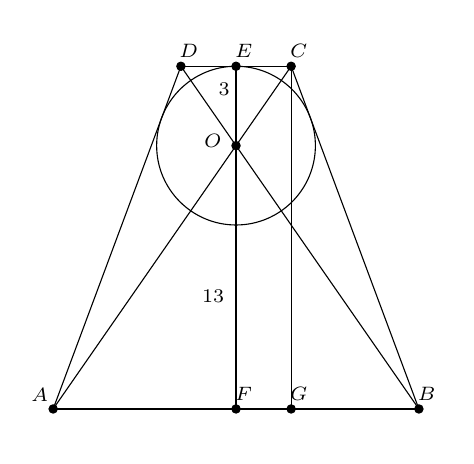
\begin{tikzpicture}[line cap=round,line join=round,x=0.7cm,y=0.7cm]
\clip(-1.78,-3.7) rectangle (5.8,3.7);
\draw(2.,1.56) circle (1.44);
\draw (1.,3.)-- (-1.317789291882535,-3.217616580310849);
\draw (-1.317789291882535,-3.217616580310849)-- (5.317789291882535,-3.2176165803108487);
\draw (1.,3.)-- (3.,3.);
\draw (3.,3.)-- (-1.317789291882535,-3.217616580310849);
\draw (1.,3.)-- (5.317789291882535,-3.2176165803108487);
\draw (3.,3.)-- (5.317789291882535,-3.2176165803108487);
\draw (2.,3.)-- (2.,-3.217616580310849);
\draw (3.,3.)-- (3.,-3.2176165803108496);
\begin{scriptsize}
\draw (1.24,-0.92) node[anchor=north west] {$13$};
\draw (1.54,2.84) node[anchor=north west] {$3$};
\draw [fill=black] (2.,3.) circle (1.5pt);
\draw[color=black] (2.14,3.28) node {$E$};
\draw [fill=black] (2.,1.56) circle (1.5pt);
\draw[color=black] (1.58,1.64) node {$O$};
\draw [fill=black] (3.,3.) circle (1.5pt);
\draw[color=black] (3.14,3.28) node {$C$};
\draw [fill=black] (1.,3.) circle (1.5pt);
\draw[color=black] (1.14,3.28) node {$D$};
\draw [fill=black] (5.317789291882535,-3.2176165803108487) circle (1.5pt);
\draw[color=black] (5.46,-2.94) node {$B$};
\draw [fill=black] (-1.317789291882535,-3.217616580310849) circle (1.5pt);
\draw[color=black] (-1.56,-2.96) node {$A$};
\draw [fill=black] (2.,-3.217616580310849) circle (1.5pt);
\draw[color=black] (2.14,-2.94) node {$F$};
\draw [fill=black] (3.,-3.2176165803108496) circle (1.5pt);
\draw[color=black] (3.14,-2.94) node {$G$};
\end{scriptsize}
\end{tikzpicture}
\end{center}

Ez az állítás belátható abból is, hogy az $ABC_{\Delta}$ egyenlő szárú, ahonnan $BC=AB=2\cdot 13x=26x$.

A $BGC$ háromszögre Pitagorasz tétele alapján felírható, hogy $16^2+(10x)^2=(26x)^2$, ahonnan $x=\dfrac{2}{3}$ következik, és így a terület:
$$t=\frac{(AB+DC)\cdot 16}{2}=\frac{(26x+6x)\cdot 16}{2}=\frac{512}{3}\text{~cm}^2.$$


\end{document}